\documentclass{standalone}
\usepackage{tikz}
\usetikzlibrary{patterns, positioning}
\usepackage[sfdefault]{ClearSans} %% option 'sfdefault' activates Clear Sans as the default text font
\usepackage[T1]{fontenc}

\begin{document}
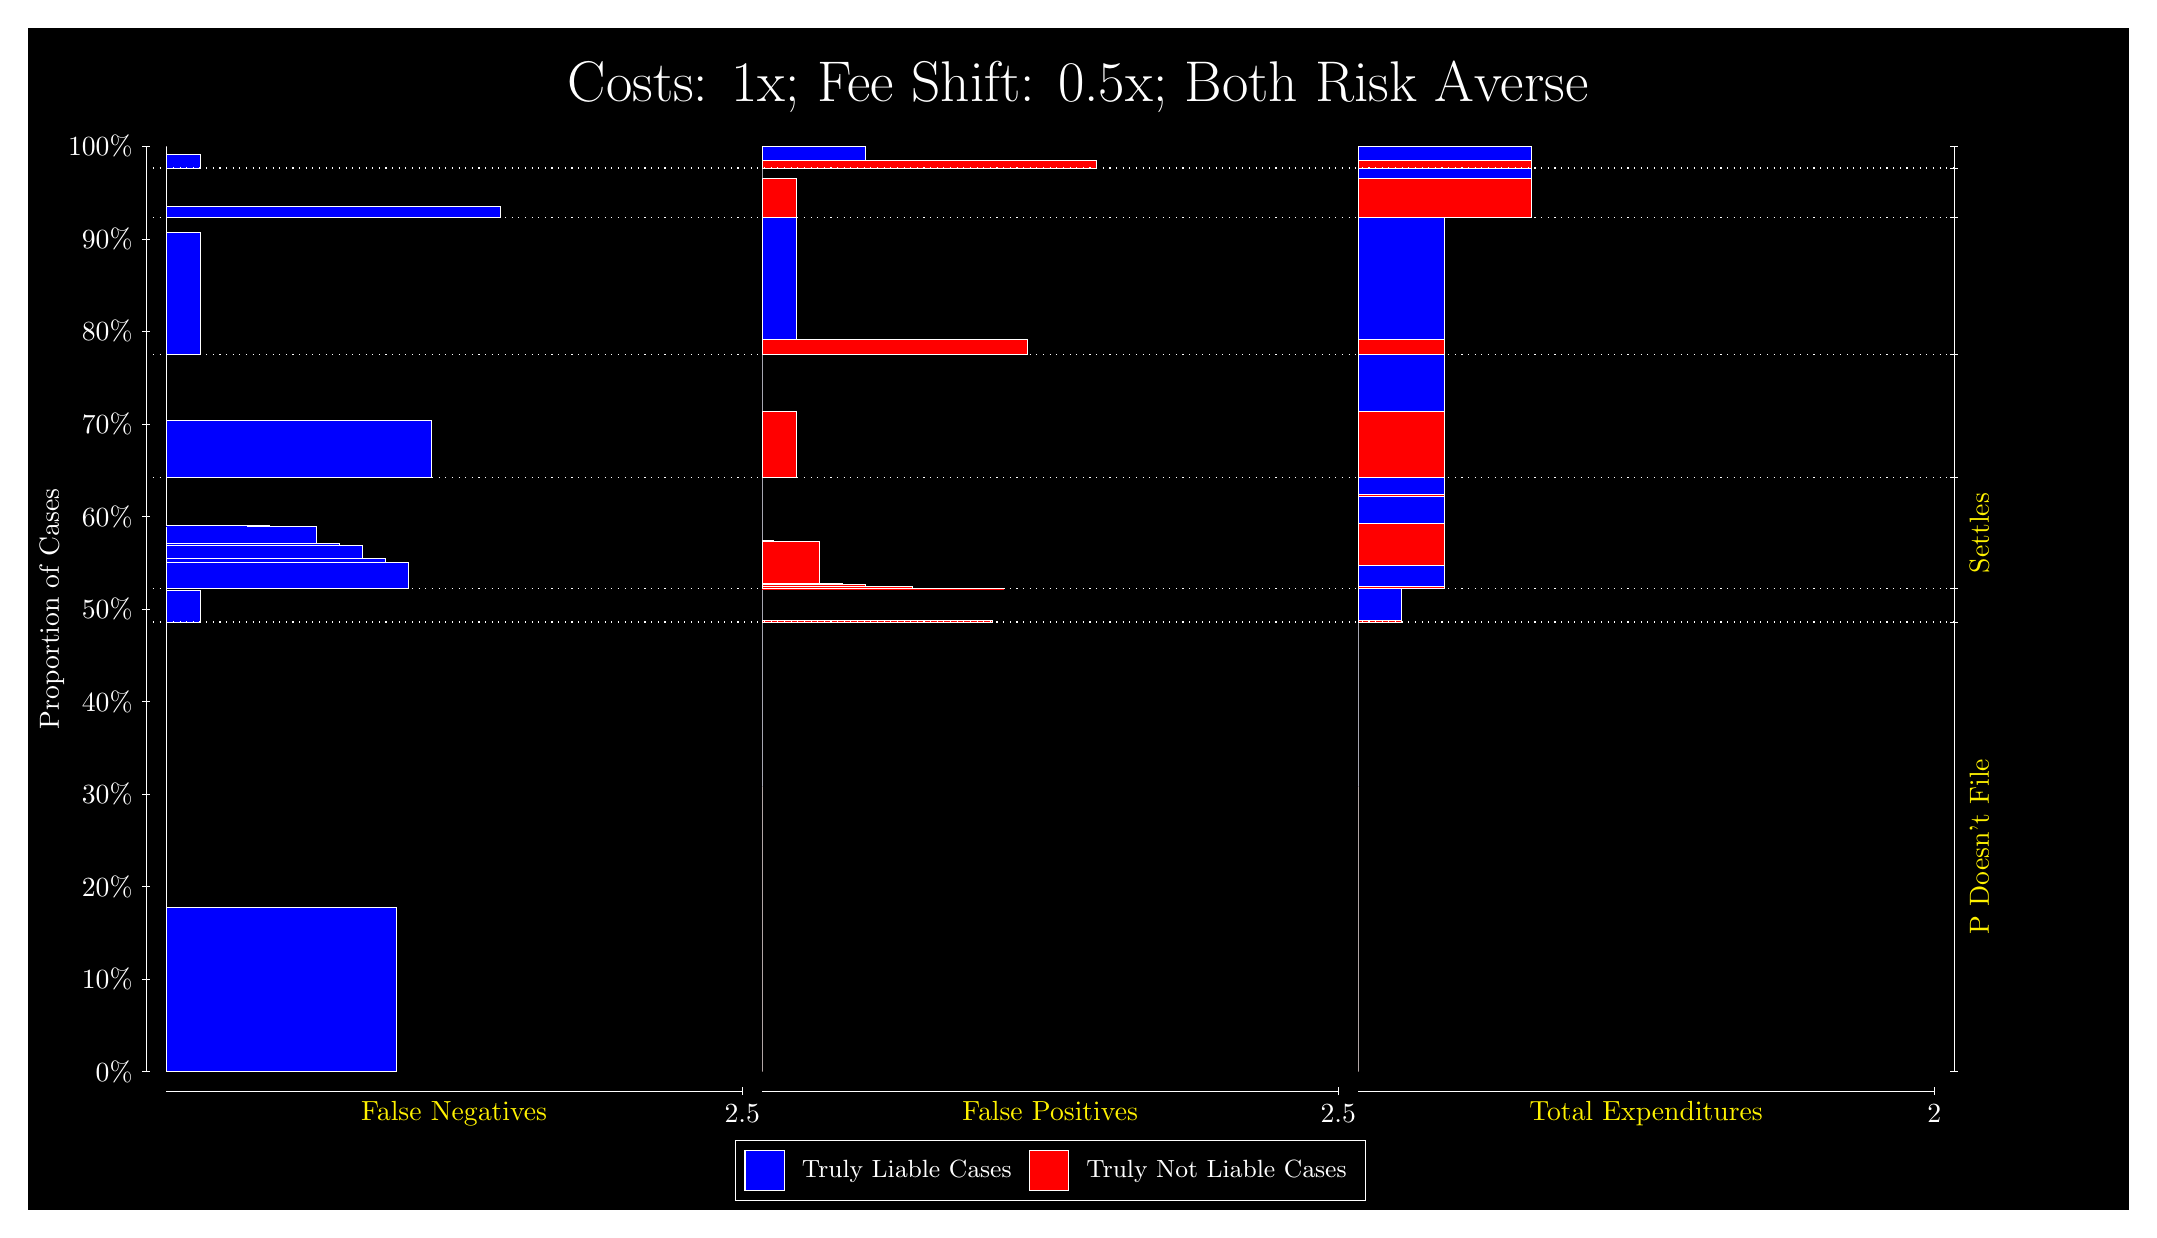
\begin{tikzpicture}
\draw[fill=black] (0,0) rectangle (26.667,15);
\draw[text=white] (0,13.5) rectangle (26.667,15) node[midway] {\huge Costs: 1x; Fee Shift: 0.5x; Both Risk Averse};
\draw[white, very thin] (1.5,1.75) -- (1.5,13.5);
\node[rotate=90, text=white, anchor=center] at (0.3, 7.625) {Proportion of Cases};
\draw[white, very thin] (1.45,1.75) -- (1.55,1.75);
\node[text=white, anchor=east] at (1.45, 1.75) {0\%};
\draw[white, very thin] (1.45,2.925) -- (1.55,2.925);
\node[text=white, anchor=east] at (1.45, 2.925) {10\%};
\draw[white, very thin] (1.45,4.1) -- (1.55,4.1);
\node[text=white, anchor=east] at (1.45, 4.1) {20\%};
\draw[white, very thin] (1.45,5.275) -- (1.55,5.275);
\node[text=white, anchor=east] at (1.45, 5.275) {30\%};
\draw[white, very thin] (1.45,6.45) -- (1.55,6.45);
\node[text=white, anchor=east] at (1.45, 6.45) {40\%};
\draw[white, very thin] (1.45,7.625) -- (1.55,7.625);
\node[text=white, anchor=east] at (1.45, 7.625) {50\%};
\draw[white, very thin] (1.45,8.8) -- (1.55,8.8);
\node[text=white, anchor=east] at (1.45, 8.8) {60\%};
\draw[white, very thin] (1.45,9.975) -- (1.55,9.975);
\node[text=white, anchor=east] at (1.45, 9.975) {70\%};
\draw[white, very thin] (1.45,11.15) -- (1.55,11.15);
\node[text=white, anchor=east] at (1.45, 11.15) {80\%};
\draw[white, very thin] (1.45,12.325) -- (1.55,12.325);
\node[text=white, anchor=east] at (1.45, 12.325) {90\%};
\draw[white, very thin] (1.45,13.5) -- (1.55,13.5);
\node[text=white, anchor=east] at (1.45, 13.5) {100\%};

\draw[white, very thin] (24.457,1.75) -- (24.457,13.5);
\draw[white, very thin] (24.407,1.75) -- (24.507,1.75);
\node[anchor=west] at (24.407, 1.75) {};
\draw[white, very thin] (24.407,7.4593) -- (24.507,7.4593);
\node[anchor=west] at (24.407, 7.4593) {};
\draw[white, very thin] (24.407,7.8827) -- (24.507,7.8827);
\node[anchor=west] at (24.407, 7.8827) {};
\draw[white, very thin] (24.407,9.2958) -- (24.507,9.2958);
\node[anchor=west] at (24.407, 9.2958) {};
\draw[white, very thin] (24.407,10.858) -- (24.507,10.858);
\node[anchor=west] at (24.407, 10.858) {};
\draw[white, very thin] (24.407,12.601) -- (24.507,12.601);
\node[anchor=west] at (24.407, 12.601) {};
\draw[white, very thin] (24.407,13.225) -- (24.507,13.225);
\node[anchor=west] at (24.407, 13.225) {};
\draw[white, very thin] (24.407,13.5) -- (24.507,13.5);
\node[anchor=west] at (24.407, 13.5) {};

\draw[white, very thin, fill=blue] (1.75,1.75) rectangle (4.6775,3.837);
\draw[white, very thin, fill=red] (1.75,3.837) rectangle (1.75,7.4593);
\draw[white, very thin, fill=blue] (1.75,7.4593) rectangle (2.1891,7.8589);
\draw[white, very thin, fill=red] (1.75,7.8589) rectangle (1.75,7.8827);
\draw[white, very thin, fill=blue] (1.75,7.8827) rectangle (4.8239,8.2174);
\draw[white, very thin, fill=blue] (1.75,8.2174) rectangle (4.5312,8.2623);
\draw[white, very thin, fill=blue] (1.75,8.2623) rectangle (4.2384,8.4272);
\draw[white, very thin, fill=blue] (1.75,8.4272) rectangle (3.9457,8.4536);
\draw[white, very thin, fill=blue] (1.75,8.4536) rectangle (3.6529,8.6754);
\draw[white, very thin, fill=blue] (1.75,8.6754) rectangle (3.3602,8.6772);
\draw[white, very thin, fill=blue] (1.75,8.6772) rectangle (3.0674,8.6813);
\draw[white, very thin, fill=blue] (1.75,8.6813) rectangle (2.7746,8.6831);
\draw[white, very thin, fill=blue] (1.75,8.6831) rectangle (2.4819,8.6931);
\draw[white, very thin, fill=red] (1.75,8.6931) rectangle (1.75,9.2958);
\draw[white, very thin, fill=blue] (1.75,9.2958) rectangle (5.1167,10.017);
\draw[white, very thin, fill=red] (1.75,10.017) rectangle (1.75,10.858);
\draw[white, very thin, fill=blue] (1.75,10.858) rectangle (2.1891,12.407);
\draw[white, very thin, fill=red] (1.75,12.407) rectangle (1.75,12.601);
\draw[white, very thin, fill=blue] (1.75,12.601) rectangle (5.9949,12.735);
\draw[white, very thin, fill=red] (1.75,12.735) rectangle (1.75,13.225);
\draw[white, very thin, fill=blue] (1.75,13.225) rectangle (2.1891,13.399);
\draw[white, very thin, fill=red] (1.75,13.399) rectangle (1.75,13.5);
\draw[white, very thin, fill=red] (9.3189,1.75) rectangle (9.3189,5.3722);
\draw[white, very thin, fill=blue] (9.3189,5.3722) rectangle (9.3189,7.4593);
\draw[white, very thin, fill=red] (9.3189,7.4593) rectangle (12.246,7.4831);
\draw[white, very thin, fill=blue] (9.3189,7.4831) rectangle (9.3189,7.8827);
\draw[white, very thin, fill=red] (9.3189,7.8827) rectangle (12.393,7.8833);
\draw[white, very thin, fill=red] (9.3189,7.8833) rectangle (12.1,7.8834);
\draw[white, very thin, fill=red] (9.3189,7.8834) rectangle (11.807,7.8836);
\draw[white, very thin, fill=red] (9.3189,7.8836) rectangle (11.515,7.8837);
\draw[white, very thin, fill=red] (9.3189,7.8837) rectangle (11.222,7.9141);
\draw[white, very thin, fill=red] (9.3189,7.9141) rectangle (10.929,7.9179);
\draw[white, very thin, fill=red] (9.3189,7.9179) rectangle (10.929,7.9179);
\draw[white, very thin, fill=red] (9.3189,7.9179) rectangle (10.636,7.9435);
\draw[white, very thin, fill=red] (9.3189,7.9435) rectangle (10.344,7.9492);
\draw[white, very thin, fill=red] (9.3189,7.9492) rectangle (10.051,8.4854);
\draw[white, very thin, fill=blue] (9.3189,8.4854) rectangle (9.4652,8.4953);
\draw[white, very thin, fill=blue] (9.3189,8.4953) rectangle (9.3189,9.2958);
\draw[white, very thin, fill=red] (9.3189,9.2958) rectangle (9.758,10.137);
\draw[white, very thin, fill=blue] (9.3189,10.137) rectangle (9.3189,10.858);
\draw[white, very thin, fill=red] (9.3189,10.858) rectangle (12.686,11.052);
\draw[white, very thin, fill=blue] (9.3189,11.052) rectangle (9.758,12.601);
\draw[white, very thin, fill=red] (9.3189,12.601) rectangle (9.758,13.091);
\draw[white, very thin, fill=blue] (9.3189,13.091) rectangle (9.3189,13.225);
\draw[white, very thin, fill=red] (9.3189,13.225) rectangle (13.564,13.326);
\draw[white, very thin, fill=blue] (9.3189,13.326) rectangle (10.636,13.5);
\draw[white, very thin, fill=red] (16.888,1.75) rectangle (16.888,5.3722);
\draw[white, very thin, fill=blue] (16.888,5.3722) rectangle (16.888,7.4593);
\draw[white, very thin, fill=red] (16.888,7.4593) rectangle (17.437,7.4831);
\draw[white, very thin, fill=blue] (16.888,7.4831) rectangle (17.437,7.8827);
\draw[white, very thin, fill=red] (16.888,7.8827) rectangle (17.986,7.9179);
\draw[white, very thin, fill=blue] (16.888,7.9179) rectangle (17.986,8.1828);
\draw[white, very thin, fill=red] (16.888,8.1828) rectangle (17.986,8.719);
\draw[white, very thin, fill=blue] (16.888,8.719) rectangle (17.986,9.0538);
\draw[white, very thin, fill=red] (16.888,9.0538) rectangle (17.986,9.0851);
\draw[white, very thin, fill=blue] (16.888,9.0851) rectangle (17.986,9.2958);
\draw[white, very thin, fill=red] (16.888,9.2958) rectangle (17.986,10.137);
\draw[white, very thin, fill=blue] (16.888,10.137) rectangle (17.986,10.858);
\draw[white, very thin, fill=red] (16.888,10.858) rectangle (17.986,11.052);
\draw[white, very thin, fill=blue] (16.888,11.052) rectangle (17.986,12.601);
\draw[white, very thin, fill=red] (16.888,12.601) rectangle (19.083,13.091);
\draw[white, very thin, fill=blue] (16.888,13.091) rectangle (19.083,13.225);
\draw[white, very thin, fill=red] (16.888,13.225) rectangle (19.083,13.326);
\draw[white, very thin, fill=blue] (16.888,13.326) rectangle (19.083,13.5);
\draw[white, dotted] (1.5,7.4593) -- (24.457,7.4593);
\draw[white, dotted] (1.5,7.8827) -- (24.457,7.8827);
\draw[white, dotted] (1.5,9.2958) -- (24.457,9.2958);
\draw[white, dotted] (1.5,10.858) -- (24.457,10.858);
\draw[white, dotted] (1.5,12.601) -- (24.457,12.601);
\draw[white, dotted] (1.5,13.225) -- (24.457,13.225);
\draw[white, very thin] (1.75,1.5) -- (9.0689,1.5);
\node[text=yellow, anchor=north] at (5.4094, 1.5) {False Negatives};
\draw[white, very thin] (9.0689,1.45) -- (9.0689,1.55);
\node[text=white, anchor=north] at (9.0689, 1.45) {2.5};

\draw[white, very thin] (9.3189,1.5) -- (16.638,1.5);
\node[text=yellow, anchor=north] at (12.978, 1.5) {False Positives};
\draw[white, very thin] (16.638,1.45) -- (16.638,1.55);
\node[text=white, anchor=north] at (16.638, 1.45) {2.5};

\draw[white, very thin] (16.888,1.5) -- (24.207,1.5);
\node[text=yellow, anchor=north] at (20.547, 1.5) {Total Expenditures};
\draw[white, very thin] (24.207,1.45) -- (24.207,1.55);
\node[text=white, anchor=north] at (24.207, 1.45) {2};

\node[text=yellow, centered, rotate=90] at (24.777, 4.6046) {P Doesn't File};

\node[text=yellow, centered, rotate=90] at (24.777, 8.5892) {Settles};





\draw (12.978300999999998,1.5) node[draw=none] (baseCoordinate) {};
\begin{scope}[align=center]
        \matrix[scale=0.5, draw=white, below=0.5cm of baseCoordinate, nodes={draw}, column sep=0.1cm]{
            \node[rectangle, draw, minimum width=0.5cm, minimum height=0.5cm, fill=blue] {}; &
            \node[draw=none, font=\small, text=white] (B) {Truly Liable Cases}; &
            \node[rectangle, draw, minimum width=0.5cm, minimum height=0.5cm, fill=red] {}; &
            \node[draw=none, font=\small, text=white] (B) {Truly Not Liable Cases}; \\
            };
\end{scope}

\end{tikzpicture}
\end{document}